\documentclass[14pt, t]{beamer}
\usepackage[T1]{fontenc}
\usepackage{graphicx, multimedia}
\usepackage{amsmath, amssymb, mathtools}
\usepackage{bm, physics}
\usepackage{siunitx}

\graphicspath{{../media}}
\sisetup{range-phrase={} to {}, separate-uncertainty=true, exponent-product=\cdot, range-units=single}


% BEGIN BIBLIOGRAPHY CONFIGURATION
% --------------------------------------------- %
\usepackage[maxcitenames = 2, backend=biber]{biblatex}
\usepackage{../bib/atlasbiblatex}
\addbibresource{../bib/sources.bib}
\renewcommand{\bibfont}{\footnotesize}
\setbeamertemplate{bibliography item}{\insertbiblabel}  % to print reference numbers and not icons
% --------------------------------------------- %
% END BIBLIOGRAPHY CONFIGURATION


% BEGIN BEAMER CONFIGURATION
% -------------------------------------- %
\setbeamertemplate{navigation symbols}{}
\usefonttheme{serif}
% \setbeamertemplate{footline}[frame number]
\setbeamertemplate{footline}{\raisebox{5.5pt}{\makebox[\paperwidth]{\hfill \makebox[20pt]{\scriptsize \insertframenumber}}}}
% -------------------------------------- %
% END BEAMER CONFIGURATION


% BEGIN CUSTOM MACROS
% --------------------------------------------- %
\definecolor{myMaroon}{RGB}{96,0,6}
\newcommand{\myhref}[2]{\hyperref[#1]{\textcolor{blue}{\underline{#2}}}}
\newcommand{\myurl}[1]{\textcolor{blue}{\texttt{\url{#1}}}}
\newcommand{\chem}[1]{\ensuremath{\mathrm{#1}}}

\newcommand{\fa}{f_{\raisebox{-0.2ex}{\scalebox{0.9}{$\mspace{-2mu} \mathrm{a}$}}}}

\newcommand{\diff}{\mathop{}\!\mathrm{d}}
\renewcommand{\vec}[1]{\bm{#1}}
\newcommand{\mat}[1]{\mathbf{#1}}
\newcommand{\tensor}[1]{\mathsf{#1}}
\newcommand{\uvec}[1]{\hat{\vec{#1}}}
\renewcommand{\grad}{\nabla}

\newcommand{\X}{\mat{X}}
\newcommand{\W}{\mat{W}}
\newcommand{\x}{\vec{x}}
\newcommand{\y}{\vec{y}}
\newcommand{\w}{\vec{w}}
\renewcommand{\b}{\vec{b}}
\newcommand{\z}{\vec{z}}
\renewcommand{\a}{\vec{a}}

\newcommand{\subgrad}[1]{\grad_{\mspace{-4mu}#1}\mspace{1mu}} % gradient with a subscript
\newcommand{\supgrad}[2]{\grad_{\mspace{-4mu}#1}\mspace{1mu}^{\mspace{-4mu}#2}} % gradient with a subscript and superscript
% --------------------------------------------- %
% END CUSTOM MACROS


\begin{document}

\begin{frame}[plain]
    \begin{center}

    \definecolor{ul-red}{RGB}{220,29,39}
    \vspace{-4mm}
    \small{\textsc{Univerza v Ljubljani}}\\
    \small{\textsc{Fakulteta za {\color{ul-red} matematiko in fiziko}}}\\[1mm]
    \footnotesize{\textsc{Oddelek za fiziko}}\\
    \vspace{2mm}
    \large{Seminar}\\
    \vspace{-2mm}
    \rule{\textwidth}{0.2pt}\\[3mm]

    
    {\Large \textbf{Neposredna klasifikacija}} \\[-1mm]
    {\small \textbf{za iskanje novih procesov}}\\[-2mm]
    {\small \textbf{v fiziki osnovnih delcev}}

    \vspace{-1mm}
    \rule{\textwidth}{0.2pt}\\[3mm]

    \vspace{5mm}

    \scriptsize{\textsc{Avtor:} Elijan Mastnak}\\
    \scriptsize{\textsc{Mentor:} prof. dr. Borut Paul Ker\v{s}evan}\\

    \end{center}
    
\end{frame}

% \begin{frame}
% \frametitle{Contents}
% \tableofcontents
% \end{frame}


\begin{frame}
    \frametitle{Kaj je klasifikacija delcev?}

    \begin{block}{Klasifikacija}
        Identifikacija \textit{produktov} trka med dvema visoko-energetskima delcema
    \end{block}

    \pause
    \vspace{2mm}
    Nas bo zanimala \textit{binarna} klasifikacija Higgsovega bozona. Produkte trkov razvrstimo v kategoriji...
    \vspace{1mm}
    \begin{enumerate}[(a)]
    
        \item Higgsov bozon (\textit{signal})

        \item karkoli drugega (\textit{ozadje})
    
    \end{enumerate}
    \vspace{-2mm}
    \begin{figure}
        \centering
        \includegraphics[width=0.65\linewidth]{vector/figures-presentation/classification.png}
    \end{figure}
    % explosion source: https://2dgameartguru.com/back-with-a-bang-creating-explosions/
\end{frame}

\begin{frame}
\frametitle{Neposredna klasifikacija}

    \begin{itemize}
    
        \item<1-> Neposredno uporablja detektorske meritve

        \item<2-> Odpravi zahtevne vmesne korake

    \end{itemize}

    \only<1>{
    \begin{figure}
        \centering
        \includegraphics[width=\linewidth]{vector/figures-slo/workflow-end-end.pdf}
    \end{figure}}
    
    \only<2>{
    \begin{figure}
        \centering
        \includegraphics[width=\linewidth]{vector/figures-slo/workflow-both.pdf}
    \end{figure}}

\end{frame}



% \begin{frame}
% \frametitle{Kaj so detektorske meritve?}

%     Nabor izmerjenih fizikalnih količin, ki opišejo produkt trka

% \vspace{2mm}
% \begin{itemize}

%     % \item Quantitative description of particle collisions

%     \item Eksperiment: Large Hadron Collider (LHC)

%     \item Detektor: Compact Muon Solenoid (CMS)

% \end{itemize}
% \vspace{4mm}
% Razložili bomo
% \begin{enumerate}

%     \item trk protonov pri eksperimentu LHC

%     \item fizikalni principi detektorja CMS

%     \item interpretacija detektorskih meritev

% \end{enumerate}
    
% \end{frame}

% \begin{frame}
%     \frametitle{Trk proton pri eksperimentu LHC}
%     \begin{columns}
%         \column{0.4\textwidth}
%         Proces:
%         \begin{enumerate}
        
%             \item vodikovi ioni

%             \item pospeševalne stopnje

%             \item LHC

%             \item trk

%             \item detektor
        
%         \end{enumerate}

%         \column{0.6\textwidth}
%         \begin{figure}[t!]
%         \centering
%         \includegraphics[width=\columnwidth]{vector/cern-complex.pdf}
%         \end{figure}
%         \vspace{-6mm}
%         \hfill
%         \tiny{prirejeno po \cite{image-cern-complex}}
        
%     \end{columns}

% \end{frame}

\begin{frame}

    \vspace{3mm}
    \begin{center}
    \makebox[\textwidth][c]{\movie{\includegraphics[width=\paperwidth]{../media/animations/collision.png}}{../media/animations/collision.ogv}}

        {\small Animacija: trk protonov v detektorju ATLAS \cite{anim-atlas}}
    \end{center}

\end{frame}

% \begin{frame}
% % some facts and figures:
% % https://www.lhc-closer.es/taking_a_closer_look_at_lhc/0.lhc_p_collisions
% % nice cern brochure in everyday language
% % https://cds.cern.ch/record/2255762/files/CERN-Brochure-2017-002-Eng.pdf

% \frametitle{rk}
%     \begin{itemize}
    
%         \item Dva protona (redko!) čelno trčita

%         \item Veriga sekundarnih procesov

%         \item Nastali delci so \textit{\color{red} decay signature}
    
%     \end{itemize}

%     \begin{figure}
%         \centering
%         \includegraphics[width=\linewidth]{vector/figures-presentation/collision.png}
%     \end{figure}
% \end{frame}



\begin{frame}

    \frametitle{Ključna omejitev}

    \begin{itemize}
    
        \item Zanimivi delci \textit{zelo} hitro razpadejo ($ \tau_{H} \sim \SI{e-22}{\second} $)

        \item \textit{Neposredna detekcija ni mogoča}

        \item Vidimo le razpadno karakteristiko
    
    \end{itemize}

    \begin{figure}
        \centering
        \includegraphics[width=\linewidth]{vector/figures-presentation/collision-question.png}
    \end{figure}

\end{frame}

% \begin{frame}
%     \frametitle{Opis {\color{red} Decay Signature}}
%     Detektor izmeri
%     \begin{itemize}
    
%         \item trajektorijo delcev (z \textit{\color{red} trackers})

%         \item energijo delcev (z \textit{kalorimetrom})
    
%     \end{itemize}
%     \vspace{5mm}
%     S pomočjo izmerkov, lahko rekonstruiramo
%     \begin{itemize}
    
%         \item identiteto delcev

%         \item gibalno količino delcev

%         \item {\color{red} production and decay vertices...}
    
%     \end{itemize}

% \end{frame}

\begin{frame}
    \frametitle{Compact Muon Solenoid}
    \begin{figure}[htb!]
        \centering
        \includegraphics[width=\linewidth]{raster/raster-svg-slo/cms-annotated.pdf}
    \end{figure}
    \vspace{-5mm}
    \tiny{vir: \cite{image-cms}}
    
\end{frame}

\begin{frame}

    \frametitle{Koordinatni sistem CMS}

    \only<1>{
        \vspace{-4mm}
    \begin{figure}[htb!]
        \centering
        \includegraphics[width=0.85\linewidth]{raster/raster-svg-slo/cms-coordinate.pdf}
    \end{figure}}

    % \only<2>{
    %     Še drugi vpogled...
    % \begin{figure}[htb!]
    %     \centering
    %     \includegraphics[width=\linewidth]{vector/figures-slo/cms-coordinate-system.pdf}
    % \end{figure}}

\end{frame}

\begin{frame}
    \frametitle{Sledilnik: merjenje trajektorije}
    
    Fizikalni principi
    \begin{itemize}

     	\item Zaporno-vezan polprevodnik
        \item Nabiti delec preleti polprevodnik
        \item Nastane par elektron-vrzel
        \item Elektron in vrzel povzročita merljivi tokovni sunek

    \end{itemize}
    \vspace{5mm}

    \pause
    Za občutek...
    \begin{itemize}
    
        % \item 13 koncentričnih plasti Si pixelov in trakov

        \item Dimenzije $ \sim \text{\SIrange{10}{100}{\micro \meter}} $

        \item $ \sim $ 75 milijon ``read-out'' kanalov

    \end{itemize}
    
\end{frame}

\begin{frame}
    \frametitle{Elektromagnetni kalorimeter (ECAL)}
    \begin{itemize}
    
        \item Meri energijo delcev

        \item Scintilatorji iz \chem{PbWO_4} % svinčevega volframata

        \item Dimenzije $ \sim \SI{2}{\centi \meter} \times \SI{2}{\centi \meter} \times \SI{20}{\centi \meter} $

        \item $ \sim $ 75\,000 scintilacijskih kristalov
    
    \end{itemize}
    \vspace{-5mm}
    \begin{figure}
        \centering
        \includegraphics[width=0.75\linewidth]{raster/png-presentation/ecal-scintillators.jpg}
    \end{figure}
    \vspace{-9mm}
    \hfill
    \tiny{vir: \cite{image-pbwo4}}
    
\end{frame}

\begin{frame}
    \frametitle{Fizikalni princip ECAL-a}
    \begin{itemize}
    
        \item Vpadni delec povzroči \textit{EM pljusk} \pause

        \item Pljusk vzbudi \chem{PbWO_4} scintilator \pause

        \item Scintilator emitira \textit{scintilacijske fotone} \pause

        \item Fotoni sprožijo \textit{fotoelektrone} v polprevodniškim fotodetektorju \pause

        \item Fotodetektor zazna tokovni sunek
    
    \end{itemize}
    \begin{equation*}
        I_{0} \propto N_{\text{e}^{-}}  \propto N_{\gamma} \propto E_{\text{dep}}
    \end{equation*}
    
\end{frame}

\begin{frame}
    \frametitle{Hadronski Kalorimeter (HCAL)}
    \begin{itemize}
    
        \item Meri energijo hadronov

        \item Medeninasti absorber in plastični scintilatorji

        \item Fizikalni principi analogi ECAL-u

    \end{itemize}

    \pause
    Zanimivost: uporaba ruskih granat iz WWII

    \hfill \tiny{vir: \cite{hcal-grenades}} \quad
    \vspace{-2.5mm}
    \begin{figure}[htb!]
        \centering
        \includegraphics[width=0.95\linewidth]{raster/png-presentation/hcal-shells}
    \end{figure}
    
\end{frame}

\begin{frame}
    
    \frametitle{Interpretacija detektorskih meritev}
    Spomnimo se, kako izgledajo detektorske meritve...
    \begin{figure}[htb!]
        \centering
        \includegraphics[width=\linewidth]{raster/raster-svg-slo/atlas.pdf}
    \end{figure}
\end{frame}


\begin{frame}
    \frametitle{Interpretacija detektorskih meritev}

    \begin{figure}[htb!]
        \centering
        \includegraphics[width=\linewidth]{raster/raster-svg-slo/event-image.pdf}
    \end{figure}
    \vspace{-9mm}
    \hfill
    {\tiny prirejeno po \cite{andrews-higgs}}

    \vspace{-1mm}
    \begin{itemize}
    
        \item mreža pixelov (analogno sliki)
        \item 2 prostorski dimenziji $ (\varphi, \theta) $
        \item 3 detektorski kanali (Tracker, ECAL, HCAL)
    
    \end{itemize}

\end{frame}

\begin{frame}
    \frametitle{Neposredna klasifikacija}

    \begin{itemize}
    
        \item Vhod: detektorske meritve (``slike trka'')

        \item Izhod: \textit{klasifikacijska napoved $ \hat{\y}_{\textup{pred}} $}
    
    \end{itemize}
    \begin{figure}[htb!]
        \centering
        \includegraphics[width=\linewidth]{raster/raster-svg-slo/cnn-in-out.png}
    \end{figure}
    
\end{frame}

% \begin{frame}
%     \frametitle{Interpretacija detektorskih meritev}
%     \begin{center}
%         \textit{Obstaja neposredna fizikalna povezava med vrednosti pixelov in trajektorijo/energijo delcev}
%     \end{center}

%     \vspace{-10mm}

%     \begin{alignat*}{3}
%         & \text{intenziteta pixelov} && \iff &&
%         \begin{cases}
%             \text{naboj v Tracker} &\\
%             \text{energija v ECAL/HCAL} &
%         \end{cases}\\[2mm]
%         & {} \hspace{2mm} \text{pozicija pixelov} && \iff && \ \text{pozicija...}
%         \begin{cases}
%             \text{Si traka} &\\
%             \text{ECAL kristala} &\\
%             \text{HCAL plošče} &
%         \end{cases}
%     \end{alignat*}
    
    
% \end{frame}

\begin{frame}
    \frametitle{Interpretacija napovedi mreže}
    \begin{itemize}
    
        \item Pravilni rezultat
        $ \vec{y} = 
        \begin{pmatrix}
            y_{\text{sig}}\\[-0.5mm]
            y_{\text{oz}}
        \end{pmatrix} $ \ {\small (iz simulacije)}

        \item Napoved: \hspace{-1.0mm}
        $ \hat{\y} = 
        \begin{pmatrix}
            \hat{y}_{\text{sig}}\\[-0.5mm]
            \hat{y}_{\text{oz}}
        \end{pmatrix} $

        \item Kategorije opišemo z vrednostmi 1 in 0
        
    \end{itemize}
    
    \begin{figure}[htb!]
        \centering
        \includegraphics[width=\linewidth]{vector/figures-slo/binary-output.pdf}
    \end{figure}
    
\end{frame}


% \begin{frame}
%     \frametitle{Tradicionalna klasifikacija}
%     \begin{enumerate}[(a)]
    
%         \item Učenje
%         \begin{itemize}
        
%             \item \textit{Simuliramo} podatke ($ \sim 10^{6} $ trkov)

%             \item Učimo nevronsko mrežo z simuliranimi podatki
        
%         \end{itemize}
%         \pause
%         \begin{center}
%         \begin{figure}[htb!]
%             \hspace{-10mm} % hack to center figure with slide and not itemize environment
%             \includegraphics[width=\linewidth]{vector/figures-slo/fcn-in-out.pdf}
%         \end{figure}    
%         \end{center}
        
%         \item Uporaba v praksi
%         \begin{itemize}
        
%             \item Rekonstruiramo kinematične količine (\textit{značilke}), ki opišejo trk ($ \vec{x}_{\text{znač}} $)

%             \item Količine vodimo v mrežo FCN

%             \item Mreža napove rezultat trka
        
%         \end{itemize}
    
%     \end{enumerate}
       
% \end{frame}



% Note to self: ``The notation $ \y $ will be consistent throughout this presentation to denote predicted classification scores!''

% START COMMENTED-OUT FCN MATERIAL
%----------------------------------------%
\iffalse
\begin{frame}
    \frametitle{Struktura mreže FCN}

    \begin{itemize}
    
        \item<1-> Hierarhija {\small (i) nevron} \ (ii) plast \ {\large (iii) mreža}

        \item<2-> Vhodna plast: sprejme podatke trka
                  
        \item<3-> Skrite plasti: večina izračunov
                  
        \item<4-> Izhodna plast: napoved kategorij
    
    \end{itemize}
    \vspace{-4mm}
    \begin{figure}[htb!]
        \centering
        \includegraphics[width=\linewidth]{vector/fcn-architecture-simple.pdf}
    \end{figure}
\end{frame}

\begin{frame}
    \frametitle{Posamezni nevron}
    \begin{itemize}
    
        \item Skalarna funkcija več spremenljivk

        \item Vhod: izhodi \textit{vseh} nevronov v prejšnji plasti

        \item Izhod: skalarna \textit{aktivacijska vrednost} $ {\color{myMaroon} a} \in \mathbb{R} $
    
    \end{itemize}
    \onslide<2->{Dva koraka:
    \begin{enumerate}[(i)]
    
        \item \textit{linearna} utežena vsota $ z = \w \cdot \a_{\text{prev}} + b $


        \item \textit{nelinearna} aktivacija $ {\color{myMaroon} a} = \fa(z) $
    
    \end{enumerate}}

    
    \begin{columns}
        \column{0.6\textwidth}
        \vspace{-8mm}
        \begin{figure}
            \centering
            \includegraphics[width=0.8\columnwidth]{vector/figures-presentation/fcn-single-neuron}
        \end{figure}

        \column{0.4\textwidth}
        \onslide<2->{
        \begin{alignat*}{3}
            \text{(i)}& \ && z \mspace{-2mu} &&= \mspace{-2mu} \bm{w} \mspace{-3mu} \cdot \mspace{-3mu} \bm{a}_{\text{prev}} \mspace{-2mu} + \mspace{-2mu} b \in \mathbb{R} \\[-0.5mm]
            \text{(ii)}& \ && {\color{myMaroon} a} \mspace{-3mu} && = \mspace{-4mu} f_{\raisebox{-0.2ex}{\scalebox{0.9}{$\mspace{-2mu} \mathrm{a}$}}}(z) \in \mathbb{R}
        \end{alignat*}}
        
    \end{columns}

\end{frame}

\begin{frame}
    \frametitle{Aktivacijska funkcija}

    \textit{Nelinearna} funkcija pred-aktivacijske vrednosti $ z $
    \begin{equation*}
        a = \fa(z) = \fa \big(\mspace{-2mu} \bm{w} \mspace{-3mu} \cdot \mspace{-3mu} \bm{a}_{\text{prev}} \mspace{-2mu} + \mspace{-2mu} b \big) \in \mathbb{R}
    \end{equation*}
    
    \only<1>{
        \vspace{-2mm}
        \begin{center}
            \textit{Nelinearna aktivacijska funkcija omogoča nelinearne odločitvene meje!}
        \end{center}
        \vspace{-1mm}
        \begin{figure}
            \centering
            \includegraphics[width=\linewidth]{vector/figures-presentation/decision-boundary}
        \end{figure}
    }

    \only<2>{
        \vspace{-6mm}
        \begin{columns}
            \column{0.57\linewidth}
            \vspace{3mm}
            \begin{itemize}
            
                \item Nekaj primerov:\\ $ \mathrm{ReLU} $ in variante, sigmoid, $ \tanh $, itd...

                \item (Večinoma) zvezno odvedljive

                \item ReLU je najpogostejši\\ v CNN

            \end{itemize}
            \column{0.55\linewidth}
            \begin{figure}[htb!]
                \centering
                \includegraphics[width=\columnwidth]{vector/relu.pdf}
            \end{figure}
        \end{columns}}
    
    
\end{frame}

\begin{frame}
    \frametitle{Plast v mreži FCN}

    \begin{itemize}
    
        \item Vektor uteži $ \w $ $ \longrightarrow $ matrika uteži $ \W $

        \item {\color{red} Bias} $ b $ $ \longrightarrow $ vektor biasov $ \b $

        \item Aktivacija $ a $ $ \longrightarrow $ vector aktivacij $ {\color{myMaroon} \a} $
    
    \end{itemize}
    
    \onslide<2->{Dva koraka:
    \begin{enumerate}[(i)]
    
        \item \textit{linearna} transformacija $ \z \mspace{-2mu} = \mspace{-2mu} \W^{\top} \mspace{-6mu} \cdot \mspace{-2mu} \bm{a}_{\text{prev}} \mspace{-2mu} + \mspace{-2mu} \b $

        \item \textit{nelinearna} aktivacija $ {\color{myMaroon} \a} = \fa (\z) $
    
    \end{enumerate}}

    \begin{columns}
        \column{0.6\textwidth}
        \vspace{-8mm}
        \begin{figure}
            \centering
            \includegraphics[width=0.8\columnwidth]{vector/figures-presentation/fcn-single-layer}
        \end{figure}

        \column{0.4\textwidth}
        \onslide<2->{
        \begin{alignat*}{3}
            \text{(i)}& \ && \z \mspace{-2mu} &&= \mspace{-2mu} \W^{\top} \mspace{-6mu} \cdot \mspace{-2mu} \bm{a}_{\text{prev}} \mspace{-2mu} + \mspace{-2mu} \b \in \mathbb{R}^{n} \\[-0.5mm]
            \text{(ii)}& \ && {\color{myMaroon} \a} \mspace{-3mu} && = \mspace{-4mu} \fa (\z) \in \mathbb{R}^{n}
        \end{alignat*}}
        
    \end{columns}

\end{frame}

\begin{frame}
    \frametitle{Kako interpretirati mrežo FCN?}

    \begin{itemize}
    
        \item $ Z $ značilk (vhod) in $ K $ kategorij (izhod)

        \item Vhod: značilke $ \x \in \mathbb{R}^{Z} $ in oznake $ \y \in \mathbb{R}^{K} $

        \item Izhod: napoved kategorij $ \hat{\y} \in \mathbb{R}^{K} $

    \end{itemize}
    \begin{center}
        \textit{FCN je vektorska funkcija $ \vec{h}: \mathbb{R}^{Z} \to \mathbb{R}^{K} $, ki jo parameterizirajo uteži $ \W^{(l)} $ in bias-i $ \b^{(l)} $.}
    \end{center}

    \pause
    \begin{block}{Cilj učenja}
        Poiskati optimalne vrednosti $ \W_{\text{opt}}^{(l)} $ in $ \b_{\text{opt}}^{(l)} $, da je napoved $ \hat{\y} = \vec{h}(\x) $ čim bližja oznaki $ \y $.
    \end{block}
    
\end{frame}

\begin{frame}
    \frametitle{Optimizacija}
    \begin{itemize}
    
        \item \textit{Izguba} $ L : \mathbb{R}^{K} \to \mathbb{R} $ \underline{vrednoti} razliko med napovedjo $ \hat{\y} $ in pravilnim odgovorom $ \y $

        \item Vhod: $ \hat{\y} \in \mathbb{R}^{K} $ $ \implies $ izhod: izguba $ L \in \mathbb{R} $

        \item Primer: \textit{\color{red} categorical cross entropy}
        \vspace{-3mm}
        \begin{equation*}
            L(\hat{\y}; \y) = - \sum_{z = 1}^{Z} y_{z} \ln \hat{y}_{z}
        \end{equation*}
    \end{itemize}
    \begin{center}
        \only<1>{\textit{Optimalne uteži in bias-e najdemo prek minimizacije funkcije izgube!}}
        \only<2>{\textit{Optimalne uteži in bias-e najdemo prek minimizacije funkcije izgube...}}
    \end{center}
    \vspace{-4mm}
    \only<2>{
    \begin{center}
        \small
        ...z uporabo numeričnih metod za več-dimenzionalne minimizacijske probleme, prilagojene na velike prostore parametrov in ogromne podatkovne baze.
    \end{center}}

\end{frame}
\fi
%----------------------------------------%
% END COMMENTED-OUT FCN MATERIAL


\begin{frame}

    \frametitle{Motivacija za konvolucijske mreže}

    Lastnosti vhodnih podatkov...
    \begin{itemize}
    
        \item več-dimenzionalnih nabori (``arrays'')

        \item ena kanalna os za različne pod-detektorje

        \item dve prostorski osi za koordinati $ \varphi $ in $ \theta $
    
    \end{itemize}
    \vspace{2mm}
    \textit{Prostorska struktura vsebuje fizikalno informacijo!}

    \begin{figure}[htb!]
        \centering
        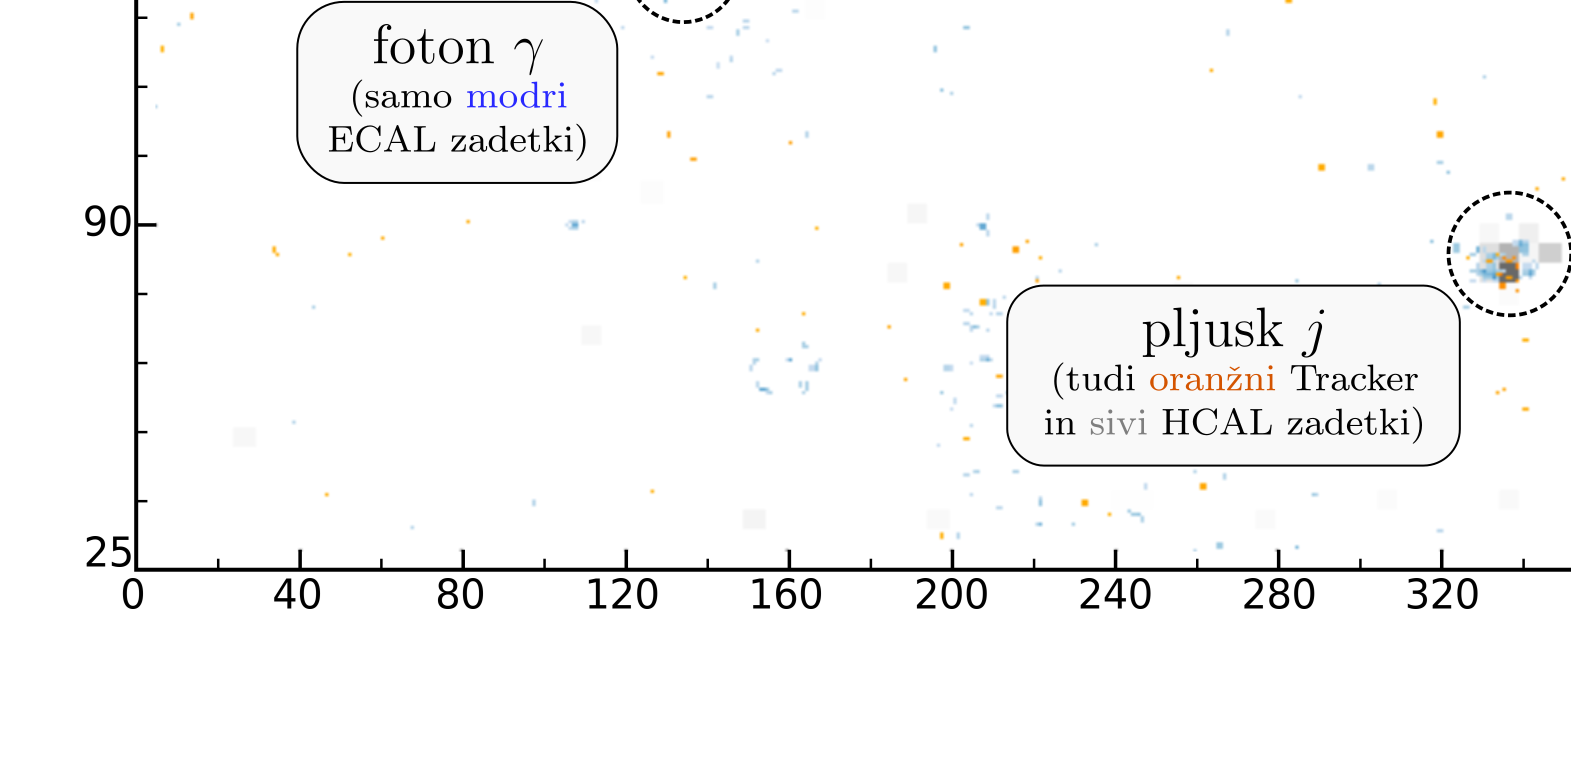
\includegraphics[width=0.85\linewidth]{raster/raster-svg-slo/event-image-cropped.pdf}
    \end{figure}   
    
\end{frame}


\begin{frame}
    \frametitle{Motivacija za konvolucijske mreže}

    % TODO box

    \only<1>{
    \begin{block}{Cilj konvolucijske mreže}
        Ohraniti in izkoristiti informacijo, vsebovana v \textit{prostorski strukturi} vhodnih podatkov.
    \end{block}}
    
    \only<2-3>{
    \begin{block}{Cilj konvolucijske mreže}
        Ohraniti in izkoristiti informacijo, vsebovana v \textit{prostorski strukturi} vhodnih podatkov...
    \end{block}}

    \onslide<2-3>{\hspace{2mm} \small{...kar klasična nevronska mreža, ki zahteva 1D vhodne podatke, ni sposobna narediti.}}

    \only<3>{
    \begin{center}
        {\large Potrebujemo torej operacijo, ki upošteva\\[-1mm] prostorsko strukturo vhodnih\\[1mm] detektorskih podatkov!}
    \end{center}}
    

\end{frame}

\begin{frame}
    \frametitle{Diskretna konvolucija}

    \vspace{5mm}

    \textit{Konvoluiramo} sliko z konvolucijskim jedrom (ang. ``kernel'')

    \begin{figure}[htb!]
        \centering
        \includegraphics[width=\linewidth]{vector/figures-slo/conv-single-channel.pdf}
    \end{figure}

\end{frame}

\begin{frame}
    \frametitle{Zgledi: diskretna konvolucija}

    \only<1>{ \vspace{10mm}
    \makebox[\textwidth][c]{\includegraphics[width=0.99\paperwidth]{vector/figures-slo/conv-single-channel-a.pdf}}}

    \only<2>{ \vspace{10mm}
    \makebox[\textwidth][c]{\includegraphics[width=0.99\paperwidth]{vector/figures-slo/conv-single-channel-b.pdf}}}

    \only<3>{ \vspace{10mm}
    \makebox[\textwidth][c]{\includegraphics[width=0.99\paperwidth]{vector/figures-slo/conv-single-channel-c.pdf}}}

    % numbers in input are pixel values, which represent deposited energy at a location in the detector

\end{frame}

\begin{frame}
    \frametitle{Posplošitve...}

    \underline{Več-kanalne slike}
    \begin{itemize}
    
        \item Vhodne slike (3D) imajo več kanalov...

        \item Torej uporabimo več-kanalno (3D) jedro!

        \item Seštejemo prek kanalne osi, da dobimo 2D izhod
    
    \end{itemize}

    \begin{figure}[htb!]
    \centering
    \includegraphics[width=\linewidth]{vector/figures-slo/conv-multi-channel.pdf}
    \end{figure}   

\end{frame}

\begin{frame}
    \frametitle{Posplošitve...}

    \underline{Več konvolucijskih jeder}
    \begin{itemize}
    
        % \item Podobno, kot več nevronov v tradicionalni mreži

        \item Vsako jedro zazna eno znacilko\\
        {\small (robovi, kontrastne barve, geometrijski liki...)}

        \item Izhod je 3D
    
    \end{itemize}

    \begin{figure}[htb!]
    \centering
    \includegraphics[width=\linewidth]{vector/figures-slo/cnn-multi-kernel.pdf}
    \end{figure}   

\end{frame}

\begin{frame}
    \frametitle{Konkretni zgledi jeder}
    
    \vspace{3mm}
    Zaznajo robove, kontrastne barve, druge vzorce...
    \vspace{-2mm}
    \begin{figure}[htb!]
        \centering
        \includegraphics[width=\linewidth]{raster/png-presentation/alexnet}
    \end{figure}
    \vspace{-9mm}
    \hfill {\tiny vir: \cite{alexnet}}
    
\end{frame}

\begin{frame}
    \frametitle{Konkretni zgledi izhodnih preslikav}

    \vspace{3mm}
    Zgledi slik, predelanih z konvolucijo:
    \vspace{-3mm}
    \begin{figure}[htb!]
        \centering
        \includegraphics[width=\linewidth]{raster/png-presentation/dogs}
    \end{figure}
    \vspace{-9mm}
    \hfill {\tiny vir: \cite{zeiler}}
    
\end{frame}

\begin{frame}
    \frametitle{(Max) Združevanje (ang. ``pooling'')}

    \vspace{3mm}
    Najbolj jasno na zgledu...

    % Cilja združevanja:
    % \vspace{2mm}
    % \begin{enumerate}[(a)]
    
    %     \item prostorsko zmanjšamo vhodne slike
    
    %     \item vpeljemo invarianco na lokalne premike

    % \end{enumerate}
    % \onslide<2->{Operacija: \textit{združevalno jedro} izpise maksimalno pixel vrednost v trenutnem vidnem polju.}
    \vspace{-1mm}
    \begin{figure}[htb!]
        \centering
        \includegraphics[width=\linewidth]{vector/figures-slo/pooling.pdf}
    \end{figure}   

\end{frame}

\begin{frame}
    \frametitle{Zgledi: max združevanje}

    \only<1>{ \vspace{10mm}
    \makebox[\textwidth][c]{\includegraphics[width=0.99\paperwidth]{vector/figures-slo/pooling-a.pdf}}}

    \only<2>{ \vspace{10mm}
    \makebox[\textwidth][c]{\includegraphics[width=0.99\paperwidth]{vector/figures-slo/pooling-b.pdf}}}

    \only<3>{ \vspace{10mm}
    \makebox[\textwidth][c]{\includegraphics[width=0.99\paperwidth]{vector/figures-slo/pooling-c.pdf}}}

    \only<4>{ \vspace{10mm}
    \makebox[\textwidth][c]{\includegraphics[width=0.99\paperwidth]{vector/figures-slo/pooling-d.pdf}}}

\end{frame}

\begin{frame}
    \frametitle{Struktura mreže CNN}
    
    \onslide<1-3>{
    Tipično zaporedje operacij:
    \begin{enumerate}[(a)]
    
        \item konvolucija

        \item nelinearna funkcija

        \item združevanje
    
    \end{enumerate}}
    \onslide<2-3>{Ponavljamo... (ni prikazano)\\}
    \onslide<3>{Sploščimo; uporabimo FCN plast za napoved}

    \only<1-2>{
    \begin{figure}[htb!]
        \centering
        \includegraphics[width=\linewidth]{vector/figures-slo/cnn-layer-sequence-a.pdf}
    \end{figure}}

    \only<3>{
    \begin{figure}[htb!]
        \centering
        \includegraphics[width=\linewidth]{vector/figures-slo/cnn-layer-sequence-b.pdf}
    \end{figure}}

\end{frame}

\begin{frame}
    \frametitle{Neposredna klasifikacija v praksi}

    Andrews et al. \textit{End-to-End Physics Event Classification with CMS Open Data}. 2020. \cite{andrews-higgs}

    \begin{itemize}
    
        \item Klasifikacija Higgsovega bozona (CMS)

        \item Signal: $ gg \to H^{0} \to \gamma \gamma $

        \item Ozadje 1: $ q \bar{q} \to \gamma \gamma $

        \item Ozadje 2: $ q \bar{q} \to \gamma j $
    
    \end{itemize}

    \begin{figure}[htb!]
        \centering
        \includegraphics[width=\linewidth]{vector/figures-slo/feynman.pdf}
    \end{figure}
    
\end{frame}

\begin{frame}
    \frametitle{Izzivi pri tej študiji}

    \begin{enumerate}[(a)]
    
        \definecolor{irrBgRed}{RGB}{175,0,0}
        \item<1-> nereducibilno ozadje 
        \begin{figure}[htb!]
            \centering
            \includegraphics[width=\linewidth]{vector/figures-presentation/feynman-irr-bg.pdf}
        \end{figure}
        \vspace{2mm}

        \item<2-> neločljivi razpadni produkti
        \begin{equation*}
            \gamma j \approx \gamma \gamma \implies \text{ozd 1} \approx \text{ozd 2} \approx \text{sig}
        \end{equation*}
    \end{enumerate}

    \vspace{7mm}

    \makebox[\textwidth]{\parbox{1.185\textwidth}{%
        
    \rule{\paperwidth}{0.3pt}\\[-5mm]
    \vspace{-5mm}
    \begin{center}
        \small{za osvežitev...}
        \vspace{-3mm}
        \begin{equation*}
            \text{sig:} \ gg \to H^{0} \to \gamma \gamma \qquad \text{ozd 1:} \ q \bar{q} \to \gamma \gamma \qquad \text{ozd 2:} \ q \bar{q} \to \gamma j
        \end{equation*}   
    \end{center}
    }}
    \vspace{-2mm}
    
\end{frame}
\begin{frame}
    \frametitle{Zgled: Klasifikacija foton-pljusk}

    Naloga: klasificirati $ gg \to H^{0} \to \gamma \gamma $ in $ q \bar{q} \to \gamma j $
    % Izziv: neločljivi razpadni produkti
    \begin{columns}

        \column{0.4\linewidth}
        \vspace{3mm}
        \begin{itemize}
    
            \item Primerjamo CNN in FCN

            \item CNN da boljše rezultate!

        \end{itemize}
        \vspace{3mm}
        Oglejmo si zakaj...

        \column{0.6\linewidth}

        \begin{figure}[htb!]
            \centering
            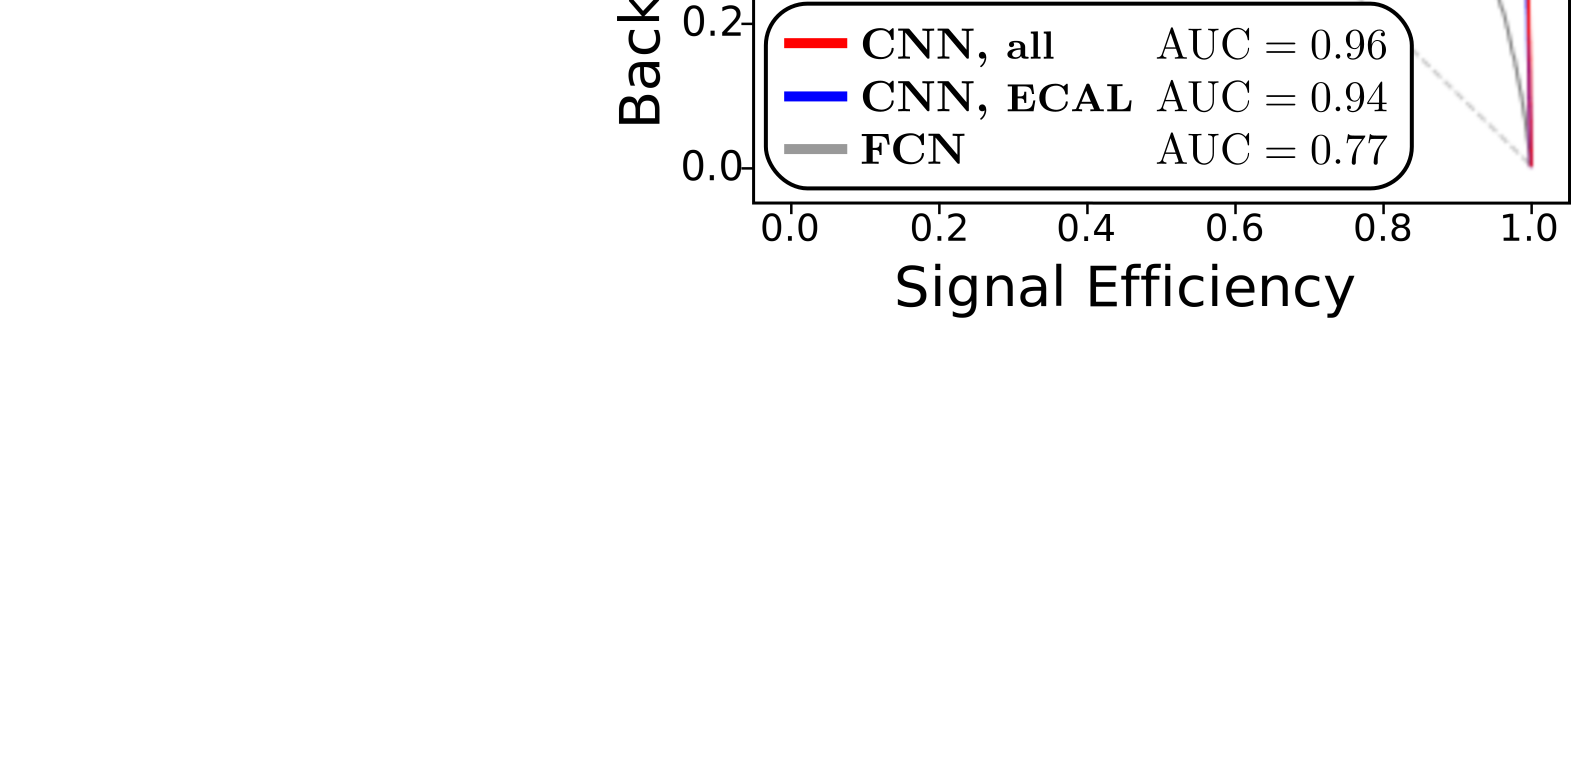
\includegraphics[width=\columnwidth]{raster/raster-svg-slo/roc.pdf}
        \end{figure}
        
    \end{columns}
    {\tiny ROC krivulja prirejena po \cite{andrews-higgs}}

\end{frame}

\begin{frame}
    \frametitle{Interpretacija rezultatov}
    Spomnimo se, kako izgledajo detektorske meritve...
    \begin{figure}[htb!]
        \centering
        \includegraphics[width=\linewidth]{raster/raster-svg-slo/event-image.pdf}
    \end{figure}
\end{frame}

\begin{frame}
    \frametitle{Interpretacija rezultatov}
    

    \only<1>{
    \begin{columns}

        \column{0.5\linewidth}
        {\centering \textbf{CNN vidi tole:}}

        \begin{figure}[htb!]
            \centering
            
\includegraphics[width=\columnwidth]{raster/raster-svg-slo/photon-jet.pdf}
        \end{figure}

        \column{0.5\linewidth}
        \hspace{8mm}\textbf{FCN vidi tole:}
        \begin{alignat*}{2}
            && p_{\text{T}} & \approx \SI{55}{\giga \electronvolt}\\
            && \varphi & \approx \ang{136} \\
            && \theta & \approx \ang{37} \\[16mm]
            && p_{\text{T}} & \approx \SI{65}{\giga \electronvolt}\\
            && \varphi & \approx \ang{335} \\
            && \theta & \approx \ang{98}
        \end{alignat*} 
    \end{columns}}

    \only<2>{
    \begin{columns}

        \column{0.5\linewidth}
        {\centering \textbf{CNN vidi tole:}}

        \begin{figure}[htb!]
            \centering
            \includegraphics[width=\columnwidth]{raster/raster-svg-slo/photon-jet-annotated.pdf}
        \end{figure}

        \column{0.5\linewidth}
        \hspace{8mm}\textbf{FCN vidi tole:}
        \begin{alignat*}{2}
            && p_{\text{T}} & \approx \SI{55}{\giga \electronvolt}\\
            && \varphi & \approx \ang{136} \\
            && \theta & \approx \ang{37} \\[16mm]
            && p_{\text{T}} & \approx \SI{65}{\giga \electronvolt}\\
            && \varphi & \approx \ang{335} \\
            && \theta & \approx \ang{98}
        \end{alignat*} 
    \end{columns}}

\end{frame}

\begin{frame}
    \frametitle{Nauk študije in zaključek}

    \begin{center}
        \textit{CNN lahko loči procese glede na distribucijo izmerkov tudi, ko je kinematika podobna.}
    \end{center}
    \underline{Lepe lastnosti neposredne klasifikacije}
    \vspace{1mm}
    \begin{itemize}
    
        \item Ohrani vso informacijo iz detektorja
        \vspace{0.5mm}

        \item Izkoristi prostorsko distribucijo dogodkov
        \vspace{0.5mm}

        \item Splošno in fleksibilno orodje
    
    \end{itemize}

    \pause
    % \vspace{1mm}
    \begin{center}
        \Large{Hvala!}
    \end{center}
    
\end{frame}

\begin{frame}[allowframebreaks]
    \frametitle{Viri}
    \printbibliography
\end{frame}

\end{document}
